\documentclass[11pt]{article}
% Shared preamble for the notes in this repository. pdfLaTeX, TeX Live 2024 or later.
\usepackage[a4paper,margin=2.6cm]{geometry}
\usepackage[T1]{fontenc}
\usepackage{lmodern}
\usepackage{microtype}
\usepackage{amsmath,amssymb,amsthm}
\usepackage{graphicx}
\usepackage{booktabs}
\usepackage{enumitem}
\usepackage[dvipsnames]{xcolor}
\usepackage[hidelinks]{hyperref}
\hypersetup{colorlinks=true,linkcolor=MidnightBlue,citecolor=MidnightBlue,urlcolor=MidnightBlue}
\graphicspath{{../../figures/}}
\setlist{itemsep=2pt,topsep=4pt}

\newtheorem{theorem}{Theorem}
\newtheorem{proposition}[theorem]{Proposition}
\newtheorem{corollary}[theorem]{Corollary}
\newtheorem{conjecture}[theorem]{Conjecture}
\theoremstyle{definition}
\newtheorem{definition}[theorem]{Definition}
% Reusable derivations, numbered note.k; each note sets \notenumber. Indexed in DERIVATIONS.md.
\newcommand{\notenumber}{0}
\newtheorem{derivation}{Derivation}
\renewcommand{\thederivation}{\notenumber.\arabic{derivation}}
\newtheorem{question}{Question}
\theoremstyle{remark}
\newtheorem{remark}[theorem]{Remark}

\newcommand{\Z}{\mathbb{Z}}
\newcommand{\Q}{\mathbb{Q}}
\newcommand{\R}{\mathbb{R}}
\newcommand{\C}{\mathbb{C}}
\newcommand{\HH}{\mathbb{H}}
\newcommand{\SL}{\mathrm{SL}}
\newcommand{\Gal}{\mathrm{Gal}}
\newcommand{\Hom}{\mathrm{Hom}}
\newcommand{\repo}{\href{https://github.com/rmorleysmith/l-functions-and-physics}{\texttt{l-functions-and-physics}}}
\newcommand{\formal}{\href{https://github.com/rmorleysmith/morley-smith-formal}{\texttt{morley-smith-formal}}}
\newcommand{\script}[1]{\href{https://github.com/rmorleysmith/l-functions-and-physics/blob/main/scripts/#1}{\texttt{scripts/#1}}}
% A path inside the Lean repository; it may break after a slash.
\newcommand{\leanpath}[1]{\nolinkurl{#1}}

% Grades used in every status table.
\newcommand{\gradeLean}{\textsc{lean}}      % proved in Lean 4 with Mathlib
\newcommand{\gradeClassical}{\textsc{classical}}  % a published theorem, cited
\newcommand{\gradeComputed}{\textsc{computed}}    % checked numerically by a script in this repository
\newcommand{\gradeConvention}{\textsc{convention}}  % a choice of units or names
\newcommand{\gradeOpen}{\textsc{open}}      % a question, conjecture or working hypothesis
% The legend printed under every status table.
\newcommand{\gradelegend}{\par\nopagebreak\smallskip\noindent\begin{minipage}{\textwidth}\small
\gradeLean: proved in Lean 4 with Mathlib.
\gradeClassical: a published theorem.
\gradeComputed: checked numerically by a script in the repository \repo.
\gradeConvention: a choice of units or names.
\gradeOpen: a question, conjecture or working hypothesis.
\end{minipage}\par\medskip}
% A plain-language physical reading, placed after each derivation.
\newcommand{\physical}{\paragraph{In physical terms.}}

\renewcommand{\notenumber}{2}

\title{Quadratic characters, lattices and waves}
\author{Richard Morley-Smith}
\date{Note 02 \quad November 2026}

\begin{document}
\maketitle

\begin{abstract}
\noindent
The quadratic Dirichlet characters $\chi_D$ of the imaginary quadratic fields appear in three physical settings.
They count the plane waves of equal frequency on a periodic lattice: for the square and hexagonal lattices and the seven other lattices of class number one, the multiplicity of a frequency is a divisor sum of $\chi_D$.
Their $L$-functions are the spectral zeta functions of those lattices and give lattice energies; the Madelung constant of the square ionic crystal is $4(\sqrt2-1)\,|\zeta(\tfrac12)|\,L(\tfrac12,\chi_{-4}) = 1.61554\ldots$, a product of two values at the centre of the critical line.
Their Gauss sums govern the diffraction of light by a grating (the Talbot effect) and the scattering of sound by Schroeder's quadratic-residue diffuser: the identity $|G(q)|^2 = q$ makes the Talbot images equally bright and the diffuser's orders equally loud, and it gives the root number of a quadratic $L$-function modulus one.
The theorems are classical; we check each numerically and pose two questions.
\end{abstract}

\section{Quadratic characters and their fields}

For a fundamental discriminant $D<0$ let $K = \Q(\sqrt D)$, with ring of integers $\mathcal O_D$, $w_D$ units and class number $h(D)$.
The Kronecker symbol $\chi_D(n) = (D/n)$ is a Dirichlet character modulo $|D|$.
It records how primes behave in $K$: a prime $p$ splits when $\chi_D(p) = 1$, stays inert when $\chi_D(p) = -1$, and ramifies when $\chi_D(p) = 0$.
Exactly nine fields have class number one (Heegner, Stark, Baker; see \cite{Cox}):
\[
  D = -3,\,-4,\,-7,\,-8,\,-11,\,-19,\,-43,\,-67,\,-163.
\]
The first two have the Eisenstein integers $\Z[\omega]$ and the Gaussian integers $\Z[i]$ as their rings of integers.
The third ring, $\Z[\tfrac{1+\sqrt{-7}}2]$, is sometimes called the Kleinian integers.

\section{Plane waves on a flat torus}

Let $\Lambda^*\subset\R^2 = \C$ be a lattice and $X$ the torus whose dual lattice is $\Lambda^*$.
The plane waves $e^{2\pi i\langle k,x\rangle}$, $k\in\Lambda^*$, are the eigenfunctions of $-\Delta$ on $X$, with eigenvalue $4\pi^2|k|^2$.
So the multiplicity of a frequency is the number of lattice points on a circle.
Take $\Lambda^* = \mathcal O_D$, where $|k|^2$ is the norm form $N(k)$.
For $D=-4$ this is $a^2+b^2$, and for $D=-3$ it is $a^2-ab+b^2$.

\begin{theorem}[Jacobi, Dirichlet]\label{thm:count}
If $h(D)=1$, the number of $k\in\mathcal O_D$ with $N(k)=n$ is
\[
  r_D(n) = w_D\sum_{d\mid n}\chi_D(d).
\]
\end{theorem}

\noindent
The divisor sum counts the ideals of norm $n$, and each ideal is principal with $w_D$ generators \cite{Cox}.
The script \script{lattice\_waves.py} checks the identity for all nine fields and all $n\le 3000$.

\physical
On a periodic membrane with the symmetry of the lattice, the number of plane waves that share a frequency is a sum of signs $\pm1$ over the divisors of $n$.
The signs record which primes split in the field.
Figure~\ref{fig:tori} shows two cases.

\begin{figure}[ht]
  \centering
  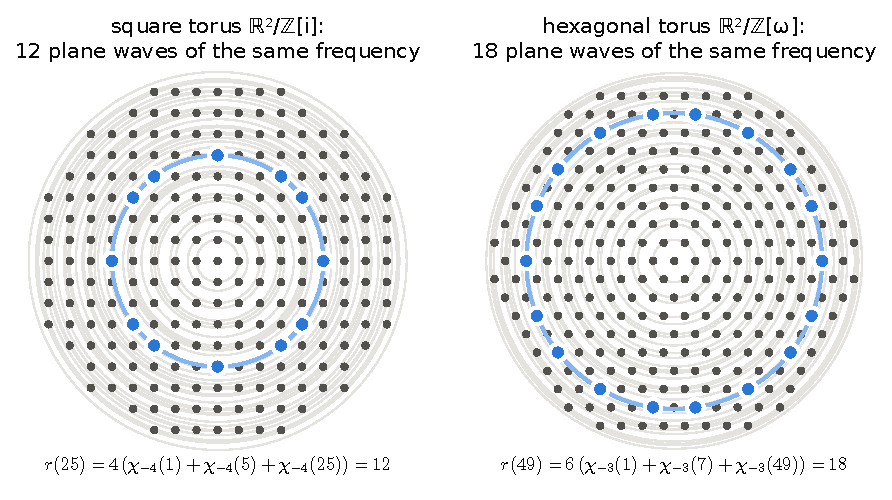
\includegraphics[width=0.9\textwidth]{waves-tori}
  \caption{Wave vectors of the same frequency lie on a circle; their number is a sum of the quadratic character. Left: $\Z[i]$, twelve waves with $|k|^2=25$. Right: $\Z[\omega]$, eighteen with $|k|^2=49$.}
  \label{fig:tori}
\end{figure}

The script checks two companions of the theorem.
\begin{itemize}
\item For class number greater than one the divisor sum counts the representations by all classes together.
For $D=-20$ the forms $x^2+5y^2$ and $2x^2+2xy+3y^2$ together represent $n$ in $2\sum_{d\mid n}\chi_{-20}(d)$ ways; the number $2$ is represented by the second form alone.
\item A square membrane with \emph{fixed} edges has modes $\sin(m\pi x)\sin(n\pi y)$ with $m,n\ge1$.
The multiplicity of $m^2+n^2=N$ is $(r_{-4}(N) - 4[N\text{ a square}])/4$.
\end{itemize}
The same count appears wherever a square or hexagonal lattice sets the wave vectors.
In the free-electron (``empty lattice'') picture of a two-dimensional crystal, plane waves whose wave vectors are reciprocal-lattice vectors of the same length are degenerate.
In powder diffraction, the Bragg reflections with the same $|G|$ fall on the same ring, and $r_D$ is their multiplicity.

\section{Spectral zeta functions and the energy of a crystal}

Summing $N(k)^{-s}$ over the lattice gives the Epstein zeta function, which is the spectral zeta function of the torus up to the factor $(4\pi^2)^{-s}$.
For class number one, Theorem~\ref{thm:count} factorises it:
\[
  Z_D(s) = \sum_{0\ne k\in\mathcal O_D} N(k)^{-s} = w_D\,\zeta(s)\,L(s,\chi_D)\qquad(\mathrm{Re}\,s>1).
\]
The script sums the lattice directly, with a disc cutoff and a tail correction.
At $s=2$ the sums agree with $w_D\zeta(2)L(2,\chi_D)$ to better than one part in $10^{6}$:

\begin{center}
\begin{tabular}{@{}lccccc@{}}
\toprule
$D$ & $-3$ & $-4$ & $-7$ & $-8$ & $-11$\\
$Z_D(2)$ & 7.71114573 & 6.02681204 & 3.78968290 & 3.50283502 & 2.99226372\\
\bottomrule
\end{tabular}
\end{center}

\noindent
For the square lattice this is $\tfrac{2\pi^2}{3}G$, with $G$ Catalan's constant.

\paragraph{The square ionic crystal.}
Put charges $\pm e$ on the points of $\Z^2$, with sign $(-1)^{x+y}$ and spacing $a$: a single layer of rock salt.
The electrostatic energy of one ion in the field of all the others is $-\alpha e^2/a$ (Gaussian units), where the Madelung constant $\alpha$ is minus the alternating sum of $(x^2+y^2)^{-1/2}$.

\begin{proposition}\label{prop:madelung}
For $\mathrm{Re}\,s>1$, and by analytic continuation,
\[
  \sum_{(x,y)\ne0}\frac{(-1)^{x+y}}{(x^2+y^2)^s} = -4\,(1-2^{1-s})\,\zeta(s)\,L(s,\chi_{-4}).
\]
At $s=\frac12$ this gives $\alpha = 4(\sqrt2-1)\,|\zeta(\tfrac12)|\,L(\tfrac12,\chi_{-4}) = 1.6155426267\ldots$
\end{proposition}

\begin{proof}
First, $(-1)^{x+y} = (-1)^{x^2+y^2}$, so the sum is $\sum_n (-1)^n r_{-4}(n) n^{-s}$.
Next, $r_{-4} = 4\,(1*\chi_{-4})$, and $\chi_{-4}$ vanishes on even numbers, so $(-1)^{dm} = (-1)^m$ whenever $\chi_{-4}(d)\neq 0$.
The sum is therefore $4L(s,\chi_{-4})\sum_m(-1)^m m^{-s} = -4L(s,\chi_{-4})(1-2^{1-s})\zeta(s)$.
\end{proof}

At $s=\tfrac12$ the lattice sum converges conditionally.
Summed over expanding squares it converges to the value given by the analytic continuation \cite{Lattice}.
The script sums squares of ions, both plainly and with Evjen's weighting (half charges on edges, quarter charges on corners) \cite{Evjen}.
At half-width 200 the weighted sum matches the formula to $10^{-5}$ (Figure~\ref{fig:madelung}).
The three-dimensional rock-salt constant, $1.7475646\ldots$, is computed the same way.
There the lattice-point counts $r_3(n)$ are class numbers rather than divisor sums (note~08), and no closed form in $L$-values is known \cite{Lattice}.

\physical
The electrostatic energy of an ion in this model crystal is a product of two $L$-values at $s=\frac12$, the centre of the critical line.

\begin{figure}[ht]
  \centering
  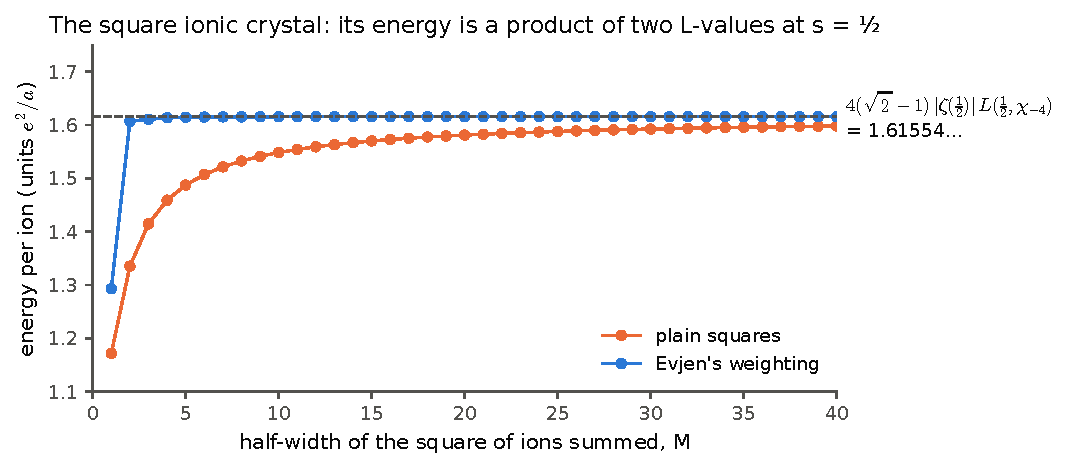
\includegraphics[width=0.82\textwidth]{waves-madelung}
  \caption{Partial sums of the Madelung constant of the square ionic crystal. Evjen's neutral weighting converges quickly to the product of $L$-values.}
  \label{fig:madelung}
\end{figure}

\section{Gauss sums: diffraction and diffusion}

The quadratic Gauss sum is $G(q) = \sum_{n\bmod q} e^{2\pi i n^2/q}$.
Gauss proved that it equals $(1+i)\sqrt q$, $\sqrt q$, $0$ or $i\sqrt q$ as $q\equiv 0,1,2,3\pmod 4$ \cite{IrelandRosen}.
For an odd prime $p$, $G(p)$ is the Gauss sum $\tau(\chi_p)$ of the Legendre symbol, so $|\tau(\chi_p)| = \sqrt p$.
The script \script{gauss\_sums\_waves.py} checks both for $q\le400$ and $p<500$.

\paragraph{The Talbot effect.}
Light of wavelength $\lambda$ passes through a grating of period $d$ with transmission $g(x) = \sum c_n e^{2\pi i n x/d}$.
In the paraxial approximation, at distance $z = u\,z_T$ with $z_T = 2d^2/\lambda$, the field is
\[
  \psi(x,u) = \sum_n c_n\,e^{2\pi i(nx/d - n^2u)}.
\]
At $u=1$ the grating reappears (Talbot, 1836 \cite{Talbot}).
At a rational distance $u=p/q$ the factor $e^{-2\pi i pn^2/q}$ depends only on $n\bmod q$.
Expanding it in additive characters gives
\[
  \psi(x,p/q) = \sum_{m\bmod q} a_m\,g\!\left(x-\tfrac{md}{q}\right),\qquad a_m = \frac1q\sum_{n\bmod q}e^{2\pi i(mn-pn^2)/q}.
\]
So the field is a sum of shifted copies of the grating, weighted by Gauss sums \cite{BerryKlein}.
Completing the square shows that $|a_m| = 1/\sqrt q$ for every $m$ when $q$ is odd: $q$ images of equal brightness.
When $q$ is even, exactly $q/2$ of the $a_m$ are non-zero, each of modulus $\sqrt{2/q}$.
The script verifies both statements and the decomposition itself for every $p/q$ with $q\le12$ (Figure~\ref{fig:talbot}).

\begin{figure}[ht]
  \centering
  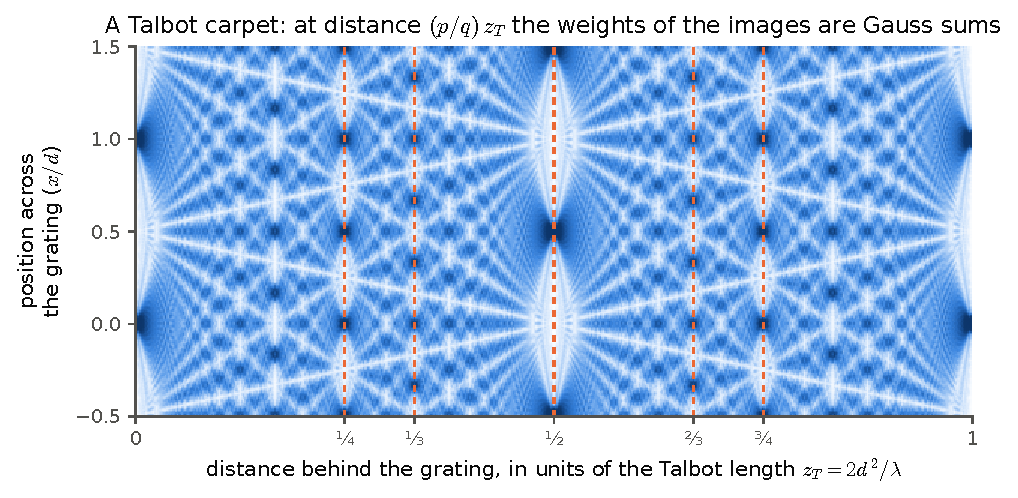
\includegraphics[width=0.92\textwidth]{waves-talbot}
  \caption{The Talbot carpet of a grating with slits one tenth of the period wide; darker shading marks higher intensity. At $\frac14$ and $\frac34$ of the Talbot length there are two images per period, at $\frac13$ and $\frac23$ three, and at $\frac12$ one, shifted by half a period.}
  \label{fig:talbot}
\end{figure}

\paragraph{Schroeder's diffuser.}
A surface of wells with depths proportional to $n^2\bmod p$ reflects a plane wave with phases $e^{2\pi i n^2/p}$ at the design frequency.
Its far field in diffraction order $m$ is proportional to $\sum_n e^{2\pi i(n^2-mn)/p}$.
Completing the square shows that this has modulus $\sqrt p$ for every $m$.
So the reflected energy is shared equally among the $p$ orders, a distribution of maximal entropy $\log p$.
Schroeder proposed these surfaces for concert halls \cite{Schroeder79, SchroederBook}, and they are still in use.
The script checks the flat spectrum for every odd prime below 200 (Figure~\ref{fig:schroeder}).

\begin{figure}[ht]
  \centering
  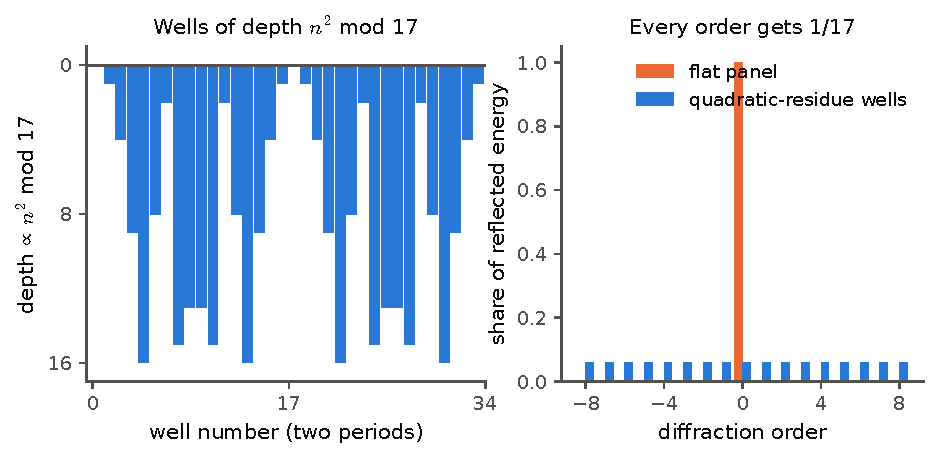
\includegraphics[width=0.9\textwidth]{waves-schroeder}
  \caption{Left: two periods of a quadratic-residue diffuser for $p=17$. Right: a flat panel sends all the energy into the specular order; the diffuser gives every order $1/17$.}
  \label{fig:schroeder}
\end{figure}

\paragraph{The root number.}
For a primitive real character $\chi$ modulo $q$ with $\chi(-1) = (-1)^a$, the completed $L$-function is
\[
  \Lambda(s,\chi) = (q/\pi)^{(s+a)/2}\,\Gamma\!\left(\tfrac{s+a}2\right)L(s,\chi).
\]
It satisfies $\Lambda(1-s,\chi) = \varepsilon(\chi)\Lambda(s,\chi)$ with root number $\varepsilon(\chi) = \tau(\chi)/(i^a\sqrt q)$ \cite{Davenport}.
The identity $|\tau(\chi)| = \sqrt q$ makes $|\varepsilon| = 1$, and for real characters Gauss's evaluation of the sign gives $\varepsilon = 1$.
The script checks the functional equation, with $\varepsilon=1$, for $\chi_{-4}$, $\chi_{-3}$, $\chi_{-7}$, $\chi_5$ and $\chi_{12}$.
So one normalisation does three jobs.
It makes the Talbot images equally bright and the diffuser's orders equally loud, and it makes the completed $L$-function symmetric about $\mathrm{Re}\,s=\frac12$.

\section{The programme, and questions}

Our working hypothesis is that the arithmetic of quadratic residues models wave propagation.
The three settings above realise it exactly, through classical theorems that the scripts check.
\begin{itemize}
\item Mode counting on lattices is the character $\chi_D$.
\item Lattice energies are values of $L(s,\chi_D)$.
\item Equal-brightness diffraction is the Gauss sum.
\end{itemize}
Two questions extend them.

\begin{question}
The lattices $\mathcal O_{-7}$ (centred rectangular, $1:\sqrt7$), $\mathcal O_{-8}$ (rectangular, $1:\sqrt2$) and $\mathcal O_{-11}$ (centred rectangular, $1:\sqrt{11}$) are realisable as two-dimensional photonic or phononic crystals.
Their empty-lattice degeneracies are predicted by $\chi_{-7}$, $\chi_{-8}$, $\chi_{-11}$.
Which of these degeneracies survive a periodic potential, which split, and is the splitting governed by the arithmetic of $\mathcal O_D$?
\end{question}

\begin{question}
The newform of weight 2 and level 11 has root number $+1$, since its Fricke eigenvalue is $-1$; both statements are proved in Lean (\formal, \texttt{tau-track/TauTrack/ElevenFunctionalEquation}).
Is there a physical system whose equal-brightness normalisation is that root number, as the Gauss sum is for the Talbot effect?
Note~10 finds one reading at level 2, where the root number is the parity of a spin state.
\end{question}

\section*{Status of the statements}

\begin{center}
\small
\begin{tabular}{@{}p{0.62\textwidth}l@{}}
\toprule
Statement & Grade\\
\midrule
Theorem~\ref{thm:count} for the nine fields, $n\le3000$; the class-number-two example & \gradeClassical{}, \gradeComputed\\
Epstein zeta factorisation; values at $s=2$ & \gradeClassical{}, \gradeComputed\\
Proposition~\ref{prop:madelung}; $\alpha = 1.6155426\ldots$ & \gradeClassical{}, \gradeComputed\\
Gauss sums; Talbot weights; Schroeder's flat spectrum & \gradeClassical{}, \gradeComputed\\
Functional equations with root number 1 for five characters & \gradeClassical{}, \gradeComputed\\
Level 11: Fricke eigenvalue $-1$ and root number $+1$ & \gradeLean\\
The working hypothesis; Questions 1 and 2 & \gradeOpen\\
\bottomrule
\end{tabular}
\end{center}
\gradelegend

\begin{thebibliography}{9}
\bibitem{BerryKlein} M.~V. Berry and S.~Klein, Integer, fractional and fractal Talbot effects, \emph{J. Mod. Opt.} 43 (1996), 2139--2164.
\bibitem{Lattice} J.~M. Borwein, M.~L. Glasser, R.~C. McPhedran, J.~G. Wan and I.~J. Zucker, \emph{Lattice Sums Then and Now}, Cambridge University Press, 2013.
\bibitem{Cox} D.~A. Cox, \emph{Primes of the Form $x^2+ny^2$}, 2nd ed., Wiley, 2013.
\bibitem{Davenport} H.~Davenport, \emph{Multiplicative Number Theory}, 3rd ed., Springer, 2000.
\bibitem{Evjen} H.~M. Evjen, On the stability of certain heteropolar crystals, \emph{Phys. Rev.} 39 (1932), 675--687.
\bibitem{IrelandRosen} K.~Ireland and M.~Rosen, \emph{A Classical Introduction to Modern Number Theory}, 2nd ed., Springer, 1990.
\bibitem{Schroeder79} M.~R. Schroeder, Binaural dissimilarity and optimum ceilings for concert halls: more lateral sound diffusion, \emph{J. Acoust. Soc. Am.} 65 (1979), 958--963.
\bibitem{SchroederBook} M.~R. Schroeder, \emph{Number Theory in Science and Communication}, 5th ed., Springer, 2009.
\bibitem{Talbot} H.~F. Talbot, Facts relating to optical science, No.~IV, \emph{Phil. Mag.} 9 (1836), 401--407.
\end{thebibliography}

\end{document}
